%-----------------------------------To Be Updated for Classroom Examples--------------
\documentclass{ResumeDesignFormat1}
\usepackage[english]{babel}
\usepackage{marginnote}
\usepackage{tikz}
\usepackage{hyperref}
\usetikzlibrary{positioning}
\usetikzlibrary{backgrounds}
\usepackage{tkz-berge}
\usepackage{sectsty}
\sectionfont{\footnotesize}
\subsectionfont{\Large}
\subsubsectionfont{\large}
\paragraphfont{\lfootnotesize}
\usepackage{pagecolor}
\definecolor{c1}{rgb}{0.858, 0.188, 0.478}
\definecolor{c2}{RGB}{219, 48, 122}
\definecolor{c3}{cmyk}{0, 0.7808, 0.4429, 0.1412}
\definecolor{c4}{gray}{0.1}
\definecolor{c5}{RGB}{142, 68, 173}
\definecolor{blueish}{rgb}{0.565,0.886,1} 
\definecolor{greenish}{rgb}{0.565,1,0.886}
\definecolor{darkgray}{rgb}{0.15,0.15,0.15} 
\definecolor{lightgray}{rgb}{0.6,0.6,0.6}
\graphicspath{{Figures/}}

\begin{document}
\pagecolor{purple!2}
%-------------------------------------------------------------------------------------------%
%----------------------------------------Contact Information--------------------------------%
%-------------------------------------------------------------------------------------------%
%-------------------------------------------------------------------------------------------%
\section{Introduction}
%----------------------------------------Figure1--------------------------------------------% 
%-------------------------------------------------------------------------------------------%
\centering
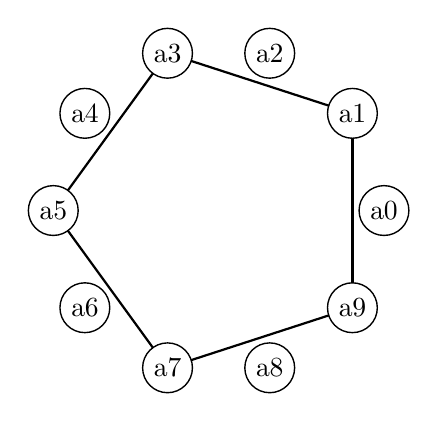
\begin{tikzpicture}[scale=0.35]
\grEmptyCycle[RA=6]{10}
\EdgeInGraphModLoop{a}{10}{2}{1}
\end{tikzpicture}
%-------------------------------------------------------------------------------------------%
%--------------------------------Summary----------------------------------------------------%
%-------------------------------------------------------------------------------------------%
\section{\centerline{\textcolor{c2}{Professional Summary}}}
%-------------------------------------------------------------------------------------------%
\input{/Summary/ProfessionalSummaryAcademic}
%-------------------------------------------------------------------------------------------%
%-------------------------------------------------------------------------------------------%
%----------------------------------------Jobs Section---------------------------------------%
%-------------------------------------------------------------------------------------------%
\section{Experience}

\begin{enumerate}
\end{enumerate}

\begin{table}[H]
\small
\centering
\begin{tabular}{p{1cm}p{1cm}p{1cm}p{1cm}}
 \hline
 Year & Company & Location & Achievements & Comments \\ 
 \hline

 \hline
\end{tabular}
\end{table}
%-------------------------------------------------------------------------------------------%
%----------------------------------------Education Section----------------------------------%
%-------------------------------------------------------------------------------------------%
\section{Education}

\begin{enumerate}
\end{enumerate}


\begin{table}[H]
\small
\centering
\begin{tabular}{p{1cm}p{1cm}p{1cm}p{1cm}}
 \hline
 Degree & Year & School & Major & Comments \\ 
 \hline

 \hline
\end{tabular}
\end{table}

%-------------------------------------------------------------------------------------------%
%------------------------Lecture Posters and Programs Section-------------------------------%
%-------------------------------------------------------------------------------------------%
\section{Lectures}
\subsection{Course 1}
\begin{enumerate}
\item \textbf{Classroom Lecture Model Series 1}: \textcolor{c2}{Lecture 1:}
\end{enumerate}
\subsection{Course 2}
\begin{enumerate}
\item \textbf{Classroom Lecture Model Series 2}: \textcolor{c2}{Lecture 1:}
\end{enumerate}
\subsection{Course 3}
\begin{enumerate}
\item \textbf{Classroom Lecture Model Series 3}: \textcolor{c2}{Lecture 1:}
\end{enumerate}

%-------------------------------------------------------------------------------------------%
%-----------------------------------------Publications Section------------------------------%
%-------------------------------------------------------------------------------------------%
\section{Publications}

\begin{enumerate}
\end{enumerate}
%-------------------------------------------------------------------------------------------%
%------------------------------Music Research Compositions Section--------------------------%
%-------------------------------------------------------------------------------------------%
\section{Music Research Compositions}

\begin{enumerate}
\end{enumerate}

%-------------------------------------------------------------------------------------------%
%-----------------Scientific Visualization Portfolio Section--------------------------------%
%-------------------------------------------------------------------------------------------%
\section{Scientific Visualization Portfolio}

\begin{enumerate}
\end{enumerate}
%-------------------------------------------------------------------------------------------%
%----------------Graphics Design:Article 1--------------------------------------------------%
%-------------------------------------------------------------------------------------------%
\footnotesize
\begin{figure}[h]
\centering
%\includegraphics[scale=0.2]{Figure3B.png}
\caption{\textcolor{c5}{\textbf{Classroom Lecture Model Series 1:}}\footnotesize  A Mathematical Model}
\label{fig:Figure1}
\end{figure}

%-------------------------------------------------------------------------------------------%
%-------------------------------------------Awards Section----------------------------------%
%-------------------------------------------------------------------------------------------%
\section{Awards and Scholarships}

\begin{enumerate}
\end{enumerate}
%-------------------------------------------------------------------------------------------%
%-------------------------------------------Hobbies Section---------------------------------%
%-------------------------------------------------------------------------------------------%
\section{Hobbies}

\begin{enumerate}
\end{enumerate}

\end{document}
